\textbf{Pour cette première partie, aucune justification n'est demandée et une seule réponse est possible par question. Pour chaque question, reportez son numéro sur votre copie et indiquez votre réponse.}

Une réponse fausse ou l'absence de réponse n'enlève aucun point.

\bigskip
\begin{minipage}[t]{0.55\linewidth}
\subsection*{Question 1}
Dans le repère ci-contre, quelles sont les coordonnées du point A ?
\end{minipage}
\hfill~
%Début tikz
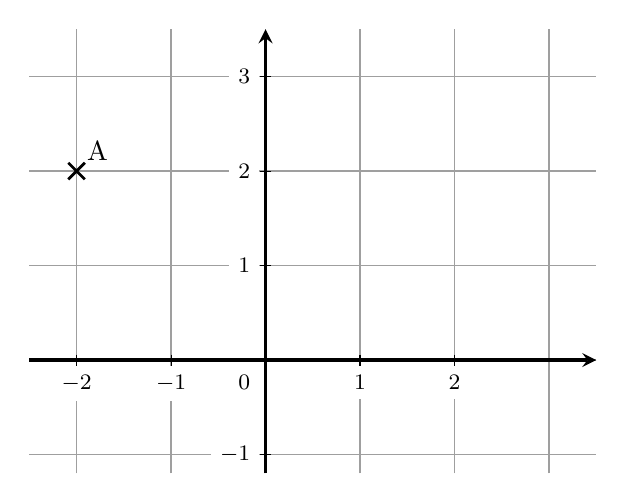
\begin{tikzpicture}[x=12mm,y=12mm,baseline={(y.base)},>=stealth]
	\draw [color = gray!75, line width = 0.5pt, xstep=1, ystep = 1] (-2.5,-1.2) grid (3.5,3.5);
	\draw[line width=1.2pt,->] (-2.5,0) -- (3.5,0);
	\foreach \x in {-2,-1,1,2}
	\draw[shift={(\x,0)},color=black] (0pt,2pt) -- (0pt,-2pt) node[below, fill = white] {\footnotesize $\np{\x}$};
	\draw[line width=1.2pt,->] (0,-1.2) -- (0,3.5);
	\foreach \y in {-1,1,2,3}
	\draw[shift={(0,\y)},color=black] (2pt,0pt) -- (-2pt,0pt) node[left, fill = white] (y) {\footnotesize $\np{\y}$};
	\draw[color=black] (-2pt,-2pt) node[below left] {{\footnotesize 0}};
	\draw[shift={(-2,2)},line width=1pt] (3pt,3pt) -- (-3pt,-3pt)
	(-3pt,3pt) -- (3pt,-3pt) (0,0) node[above right] {A};
\end{tikzpicture} \hfill~
%Fin tikz
%%Début PSTricks
%\psset{unit=1cm,arrowsize=2pt 3}
%\begin{pspicture*}(-2.5,-1.1)(2.5,3.5)
%	\psaxes[linewidth=1.25pt,labelFontSize=\scriptstyle]{->}(0,0)(-2.5,-1.1)(2.5,3.5)
%	\psgrid[gridlabels=0,subgriddiv=1,gridwidth=0.2pt](-3,-1.)(3,4)
%	\psdots(-2,2)\uput[ul](-2,2){A}
%\end{pspicture*}
%%Fin PSTricks

\medskip

\begin{minipage}[b]{0.55\linewidth}
\subsection*{Question 2}
	Dans le quadrillage ci-contre, quel est le symétrique du point K par la symétrie centrale de centre O ?
\end{minipage}\hfill~
%Début tikz
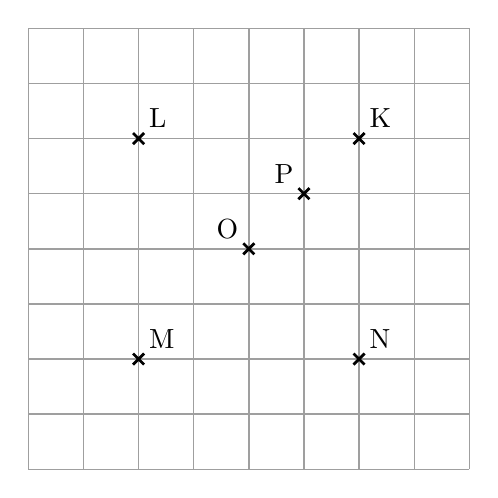
\begin{tikzpicture}[x=7mm,y=7mm,baseline={(current bounding box.center)}]
	\draw [color = gray!75, line width = 0.5pt, xstep=1, ystep = 1] (0,0) grid (8,8);
	\foreach \coordonnees/\nom/\pos in
	{{(6,6)}/K/{above right},
	{(2,2)}/M/{above right},
	{(6,2)}/N/{above right},
	{(2,6)}/L/{above right},
	{(4,4)}/O/{above left},
	{(5,5)}/P/{above left}}
		{\draw[shift=\coordonnees,line width=1pt] (2pt,2pt) -- (-2pt,-2pt)
			(-2pt,2pt) -- (2pt,-2pt) (0,0) node[\pos] {\nom};}
\end{tikzpicture}\hfill~
%Fin tikz
%%Début PSTricks
%\begin{minipage}{0.3\linewidth}
%	\psset{unit=0.5cm}
%	\begin{pspicture}(8,8)
%		\psgrid[gridlabels=0pt,subgriddiv=1,gridwidth=0.5pt]
%		\psdots(2,2)(2,6)(4,4)(5,5)(6,2)(6,6)
%		\uput[ul](2,2){M}\uput[ul](2,6){L}\uput[ul](4,4){O}\uput[ul](5,5){P}\uput[ul](6,6){K}
%	\end{pspicture}
%\end{minipage}
%%Fin PSTricks


\medskip

\begin{minipage}[t]{0.55\linewidth}
\subsection*{Question 3}
	On souhaite connaitre l'aire du triangle ABC représenté ci-contre.

	Quel calcul doit-on effectuer ?

	\begin{tblr}{colspec = {*2{X}}}
		\textbf{A.}\quad AB + BC + AC &
		\textbf{B.}\quad AC $\times$ BD $\div$ 2\\
		\textbf{C.}\quad AB $\times$ BC $\times$ CA	&
		\textbf{D.}\quad AC $\times$ BD	\\
	\end{tblr}
\end{minipage}\hfill~
%%Début tikz
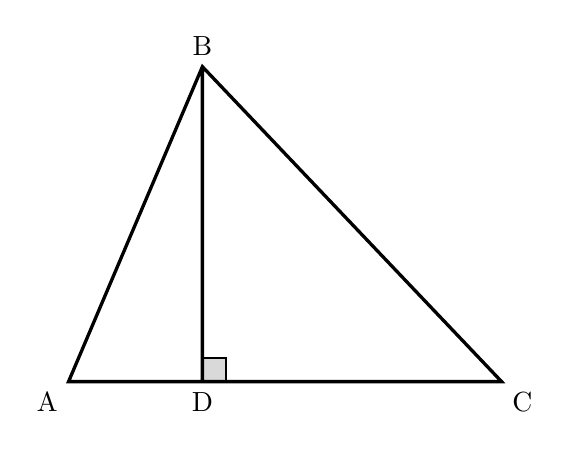
\begin{tikzpicture}[baseline={(B.base)}]
	\draw[fill=gray!30] (0,0) rectangle (0.3,0.3) ;
	\draw[line width=1.2pt]
	(-1.7,0) node[below left] {A}--
	(0,4)    node[above] (B)  {B}--
	(3.8,0)  node[below right]{C}--cycle
	(0,0)    node[below ]     {D}--(0,4);
\end{tikzpicture}
%%Fin tikz
%%%Début PSTricks
%\begin{minipage}{0.35\linewidth}
%	\psset{unit=0.9cm}
%	\begin{pspicture}(5.8,4.3)
%		\pspolygon(1.7,3.9)(0.3,0.3)(5.3,0.3)(1.7,3.9)(1.7,0.3)%BACBD
%		\uput[dl](0.3,0.3){A} \uput[u](1.7,3.9){B} \uput[dr](5.3,0.3){C} \uput[d](1.7,0.3){D}
%	\end{pspicture}
%\end{minipage}
%%%Fin PSTricks

\subsection*{Question 4}
	On lance 10 fois une pièce de monnaie.

	Les résultats obtenus sont les suivants : \emph{pile, pile, face, pile, face, face, face, face, pile, face}.

	Quelle est la fréquence d'apparition de \og \emph{pile} \fg ?

	\begin{tblr}{*{4}{X}}
		\textbf{A.}\quad $\dfrac{1}{2}$ &
		\textbf{B.}\quad $\dfrac{6}{10}$ &
		\textbf{C.}\quad $\dfrac{4}{10}$ &
		\textbf{D.}\quad $\dfrac{4}{6}$ \\
	\end{tblr}

\subsection*{Question 5}
	On note $n$ un nombre entier.

	Parmi les propositions suivantes, quelle expression donne la moitié de $n$ ?

	\begin{tblr}{*{4}{X}}
		\textbf{A.}\quad $2n$ &
		\textbf{B.}\quad $n^2$ &
		\textbf{C.}\quad $n + 2$ &
		\textbf{D.}\quad $\dfrac{n}{2}$
	\end{tblr}

\subsection*{Question 6}
	Parmi les propositions suivantes, quelle durée correspond à $\dfrac{1}{10}$ d'heure ?

	\begin{tblr}{*{4}{X}}
		\textbf{A.}\quad 0,1 min &
		\textbf{B.}\quad 1 min &
		\textbf{C.}\quad 6 min &
		\textbf{D.}\quad 10 min
	\end{tblr}

\subsection*{Question 7}
	On donne la série suivante : 10 ; 10 ; 12 ; 16.

	Calculer la moyenne de cette série.

\medskip

\begin{minipage}{0.55\linewidth}
	\subsection*{Question 8}
	La figure ci-contre n'est pas en vraie grandeur. Quelle est la valeur de $x$ ?
\end{minipage}\hfill~
%Début tikz
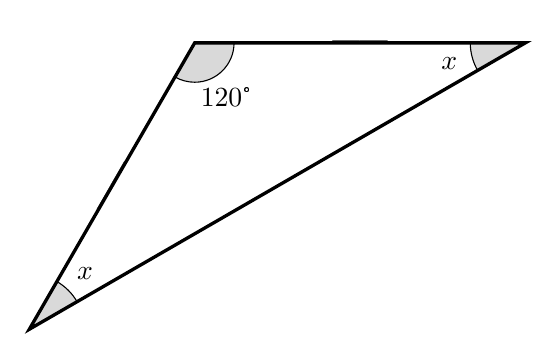
\begin{tikzpicture}[baseline={(current bounding box.center)}]
	\draw[fill=gray!30] (0,0)--(0.5,0) arc (0:-120:0.5)--cycle (-60:0.8) node{120\textdegree};
	\draw[fill=gray!30,shift={(4.2,0)}] (0,0)--(-0.7,0) arc (180:210:0.7)--cycle (195:1) node(A){$x$};
	\draw[fill=gray!30,shift={(-120:4.2)}] (0,0)--(30:0.7) arc (30:60:0.7)--cycle (45:1) node{$x$};
	\draw[line width=1.2pt] (0,0) -- (4.2,0) node[pos=0.5]{||}-- (-120:4.2)--cycle node[pos=0.5,sloped]{||};
	\end{tikzpicture}
%Fin tikz
%%Début PSTricks
%\begin{minipage}{0.37\linewidth}
%\psset{unit=0.9cm}
%\begin{pspicture}(-2,0.1)(4,-3.5)
%	\pspolygon(4;0)(0;0)(4;240)
%	\def\barre{\psline(-0.05,-0.1)(-0.05,0.1)\psline(0.05,-0.1)(0.05,0.1)}
%	\rput(2,0){\barre}\rput{60}(2;240){\barre}
%	\psarc(0;0){0.6}{-120}{0}
%	\psarc(4;240){0.4}{30}{60}\rput(-1.5,-3){$x$}
%	\psarc(4;0){0.4}{180}{210}\rput(3.35,-0.18){$x$}
%	\rput(1;-60){$120\degres$}
%\end{pspicture}
%\end{minipage}
%%Fin PSTricks

\subsection*{Question 9}

Un vélo roule à la vitesse moyenne de \np[km/h]{20}.

Quelle est la durée d'un trajet de \np[km]{15} ?

\needspace{10\baselineskip}
% saut de page si moins de 10 lignes disponibles
